% Figuras do roteiro da aula de árvores rubro-negras, no desenho de Sedgewick:
% a cor pertence à ligação que chega ao nó, e a ligação vermelha é o traço
% grosso vermelho. Cada tikzpicture vira uma página do PDF e um SVG (ver
% Makefile).

\documentclass[tikz, border=6pt]{standalone}
\usepackage[T1]{fontenc}
\usepackage[utf8]{inputenc}
\usepackage{forest}
\usetikzlibrary{backgrounds, shapes.geometric, arrows.meta, positioning, calc}

\tikzset{
  no/.style = {circle, draw=black, fill=white, text=black, inner sep=0pt,
    minimum size=1.8em, line width=0.6pt, font=\sffamily\small},
  lv/.style = {draw=red!80!black, line width=2.2pt},
  lp/.style = {draw=black, line width=0.6pt},
  sub/.style = {regular polygon, regular polygon sides=3, draw=black,
    fill=black!8, minimum size=1.1cm, inner sep=0pt, line width=0.6pt},
  bno/.style = {draw=black, fill=black!5, font=\sffamily\small,
    inner sep=4pt, line width=0.6pt},
  every picture/.style = {background rectangle/.style={fill=white},
    show background rectangle},
  bsep/.style = {draw=black, fill=white, font=\sffamily\small,
    inner sep=4pt, line width=0.6pt, dashed},
  rot/.style = {font=\sffamily\small, align=center},
  seta/.style = {-{Stealth[length=3mm]}, line width=1.2pt, draw=black!45},
  prox/.style = {-{Stealth[length=2mm]}, line width=0.6pt}
}

% Chaves de um nó de árvore B separadas por barras: \ch{1}{2}{3}.
\newcommand{\sep}{\,\textbar\,}
\newcommand{\vm}[1]{\textcolor{red!80!black}{\textbf{#1}}}

% Inserção em árvore 2-3, compartilhada com os slides.
% Inserção em árvore 2-3, com as chaves 20, 30, ..., 80 inseridas em ordem.
% Fonte única das figuras: o figuras.tex (SVG do roteiro) e os slides em
% ../00_rn_b_tries/rn_b_tries.tex dão \input neste arquivo e usam as macros
% \arvDoisTresA a \arvDoisTresD, uma por caso.
%
% O nó temporário de três chaves, que a árvore 2-3 não admite e a 2-3-4
% admite, tem borda vermelha tracejada. A chave que sobe está em vermelho.

\tikzset{
  a23/.style = {draw=black, fill=black!5, font=\sffamily\small,
    inner sep=4pt, line width=0.6pt},
  a23tmp/.style = {a23, draw=red!80!black, fill=red!6, dashed,
    line width=1pt},
  a23lig/.style = {draw=black, line width=0.6pt},
  a23seta/.style = {-{Stealth[length=3mm]}, line width=1.2pt, draw=black!45},
  a23rot/.style = {font=\sffamily\footnotesize, align=center}
}

\newcommand{\aS}{\,\textbar\,}
\newcommand{\aV}[1]{\textcolor{red!80!black}{\textbf{#1}}}

% Caso A: folha com uma chave recebe o 30.
\newcommand{\arvDoisTresA}{%
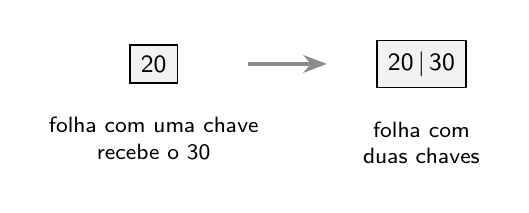
\begin{tikzpicture}
  \node [a23] (a) at (0,0) {20};
  \node [a23rot, below=3mm of a] {folha com uma chave\\recebe o 30};
  \draw [a23seta] (1.2,0) -- (2.2,0);
  \node [a23] (b) at (3.4,0) {20\aS 30};
  \node [a23rot, below=3mm of b] {folha com\\duas chaves};
\end{tikzpicture}}

% Caso B: raiz com duas chaves recebe o 40 e se divide.
\newcommand{\arvDoisTresB}{%
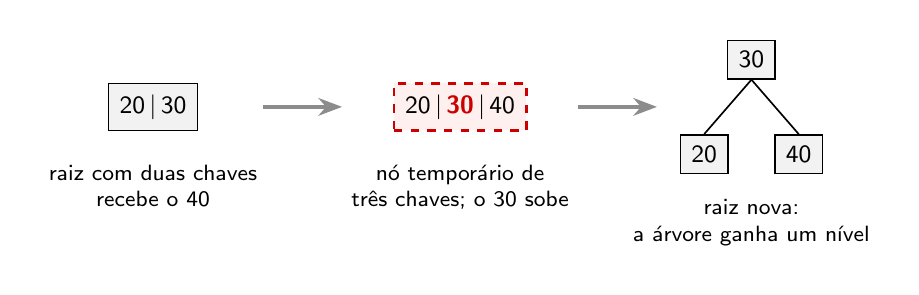
\begin{tikzpicture}
  \node [a23] (a) at (0,0) {20\aS 30};
  \node [a23rot, below=3mm of a] {raiz com duas chaves\\recebe o 40};
  \draw [a23seta] (1.4,0) -- (2.4,0);
  \node [a23tmp] (b) at (3.9,0) {20\aS \aV{30}\aS 40};
  \node [a23rot, below=3mm of b] {nó temporário de\\três chaves; o 30 sobe};
  \draw [a23seta] (5.4,0) -- (6.4,0);
  \node [a23] (r) at (7.6,0.6) {30};
  \node [a23] (e) at (7,-0.6) {20};
  \node [a23] (d) at (8.2,-0.6) {40};
  \draw [a23lig] (r.south) -- (e.north);
  \draw [a23lig] (r.south) -- (d.north);
  \node [a23rot, below=2mm of $(e.south)!0.5!(d.south)$] {raiz nova:\\a árvore ganha um nível};
\end{tikzpicture}}

% Caso C: folha com duas chaves e pai com uma; entra o 60.
\newcommand{\arvDoisTresC}{%
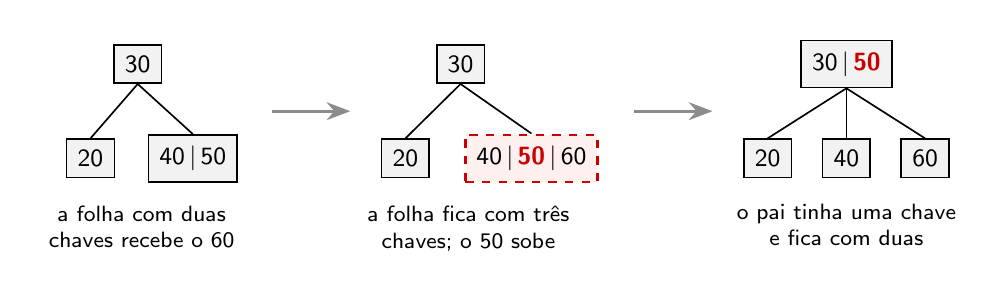
\begin{tikzpicture}
  \begin{scope}
    \node [a23] (r) at (0.6,0.6) {30};
    \node [a23] (e) at (0,-0.6) {20};
    \node [a23] (d) at (1.3,-0.6) {40\aS 50};
    \draw [a23lig] (r.south) -- (e.north);
    \draw [a23lig] (r.south) -- (d.north);
    \node [a23rot, below=2mm of $(e.south)!0.5!(d.south)$] {a folha com duas\\chaves recebe o 60};
  \end{scope}
  \draw [a23seta] (2.3,0) -- (3.3,0);
  \begin{scope}[xshift=4cm]
    \node [a23] (r) at (0.7,0.6) {30};
    \node [a23] (e) at (0,-0.6) {20};
    \node [a23tmp] (d) at (1.6,-0.6) {40\aS \aV{50}\aS 60};
    \draw [a23lig] (r.south) -- (e.north);
    \draw [a23lig] (r.south) -- (d.north);
    \node [a23rot, below=2mm of $(e.south)!0.5!(d.south)$] {a folha fica com três\\chaves; o 50 sobe};
  \end{scope}
  \draw [a23seta] (6.9,0) -- (7.9,0);
  \begin{scope}[xshift=8.6cm]
    \node [a23] (r) at (1,0.6) {30\aS \aV{50}};
    \node [a23] (e) at (0,-0.6) {20};
    \node [a23] (m) at (1,-0.6) {40};
    \node [a23] (d) at (2,-0.6) {60};
    \foreach \f in {e, m, d} \draw [a23lig] (r.south) -- (\f.north);
    \node [a23rot, below=2mm of m.south] {o pai tinha uma chave\\e fica com duas};
  \end{scope}
\end{tikzpicture}}

% Caso D: folha e pai com duas chaves; entra o 80 e a divisão sobe até a raiz.
\newcommand{\arvDoisTresD}{%
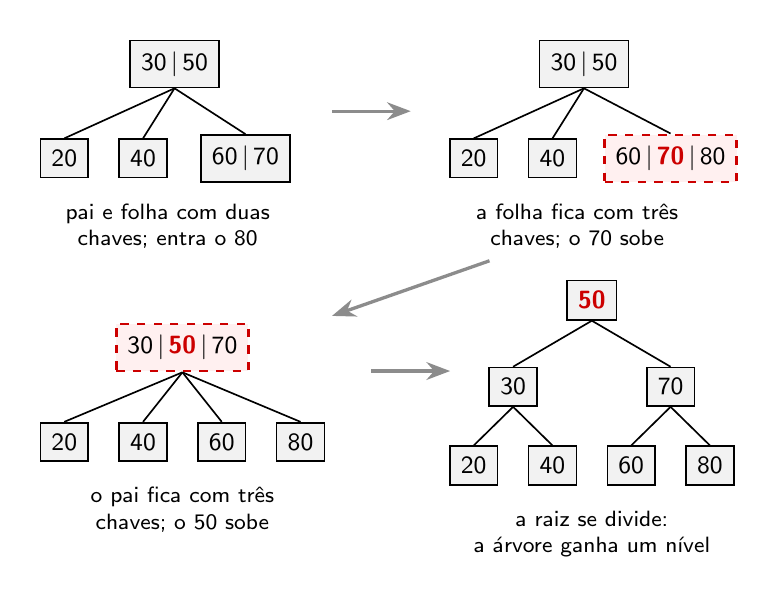
\begin{tikzpicture}
  \begin{scope}
    \node [a23] (r) at (1.4,0.6) {30\aS 50};
    \node [a23] (f1) at (0,-0.6) {20};
    \node [a23] (f2) at (1,-0.6) {40};
    \node [a23] (f3) at (2.3,-0.6) {60\aS 70};
    \foreach \f in {f1, f2, f3} \draw [a23lig] (r.south) -- (\f.north);
    \node [a23rot, below=2mm of f2.south east] {pai e folha com duas\\chaves; entra o 80};
  \end{scope}
  \draw [a23seta] (3.4,0) -- (4.4,0);
  \begin{scope}[xshift=5.2cm]
    \node [a23] (r) at (1.4,0.6) {30\aS 50};
    \node [a23] (f1) at (0,-0.6) {20};
    \node [a23] (f2) at (1,-0.6) {40};
    \node [a23tmp] (f3) at (2.5,-0.6) {60\aS \aV{70}\aS 80};
    \foreach \f in {f1, f2, f3} \draw [a23lig] (r.south) -- (\f.north);
    \node [a23rot, below=2mm of f2.south east] {a folha fica com três\\chaves; o 70 sobe};
  \end{scope}
  \draw [a23seta] (5.4,-1.9) -- (3.4,-2.6);
  \draw [a23seta] (3.9,-3.3) -- (4.9,-3.3);
  \begin{scope}[yshift=-3.6cm]
    \node [a23tmp] (r) at (1.5,0.6) {30\aS \aV{50}\aS 70};
    \node [a23] (f1) at (0,-0.6) {20};
    \node [a23] (f2) at (1,-0.6) {40};
    \node [a23] (f3) at (2,-0.6) {60};
    \node [a23] (f4) at (3,-0.6) {80};
    \foreach \f in {f1, f2, f3, f4} \draw [a23lig] (r.south) -- (\f.north);
    \node [a23rot, below=2mm of $(f2.south)!0.5!(f3.south)$] {o pai fica com três\\chaves; o 50 sobe};
  \end{scope}
  \begin{scope}[xshift=5.2cm, yshift=-3.6cm]
    \node [a23] (r) at (1.5,1.2) {\aV{50}};
    \node [a23] (i1) at (0.5,0.1) {30};
    \node [a23] (i2) at (2.5,0.1) {70};
    \draw [a23lig] (r.south) -- (i1.north);
    \draw [a23lig] (r.south) -- (i2.north);
    \node [a23] (f1) at (0,-0.9) {20};
    \node [a23] (f2) at (1,-0.9) {40};
    \node [a23] (f3) at (2,-0.9) {60};
    \node [a23] (f4) at (3,-0.9) {80};
    \draw [a23lig] (i1.south) -- (f1.north);
    \draw [a23lig] (i1.south) -- (f2.north);
    \draw [a23lig] (i2.south) -- (f3.north);
    \draw [a23lig] (i2.south) -- (f4.north);
    \node [a23rot, below=2mm of $(f2.south)!0.5!(f3.south)$] {a raiz se divide:\\a árvore ganha um nível};
  \end{scope}
\end{tikzpicture}}


\begin{document}

% 1. Exemplo da aula: 50 30 90 20 40 95 10 35 45 inseridos em ordem.
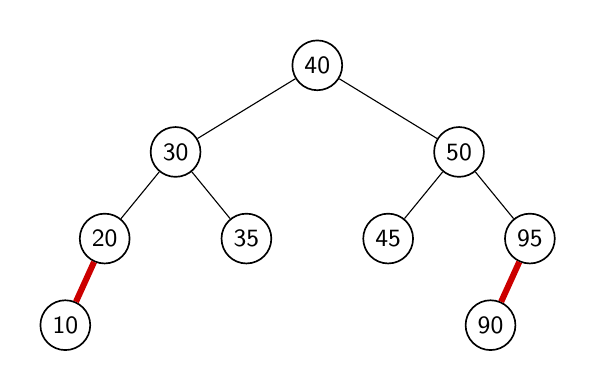
\begin{tikzpicture}[level distance=1.1cm,
    level 1/.style={sibling distance=3.6cm},
    level 2/.style={sibling distance=1.8cm},
    level 3/.style={sibling distance=1cm}]
  \node [no] {40}
  child { node [no] {30}
      child { node [no] {20}
          child { node [no] {10} edge from parent [lv] }
          child [missing]
        }
      child { node [no] {35} }
    }
  child { node [no] {50}
      child { node [no] {45} }
      child { node [no] {95}
          child { node [no] {90} edge from parent [lv] }
          child [missing]
        }
    };
\end{tikzpicture}

% 2. Nó 2-3 com duas chaves e a representação binária correspondente.
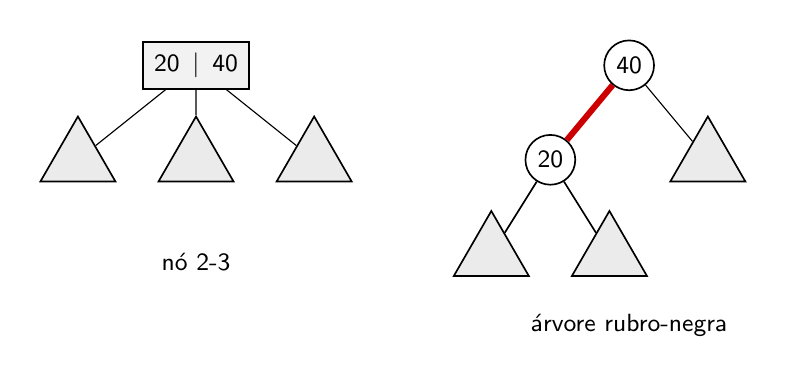
\begin{tikzpicture}[level distance=1.2cm]
  \node [bno] at (0,0) {20 \,\textbar\, 40}
    [level 1/.style={sibling distance=1.5cm}]
    child { node [sub] {} }
    child { node [sub] {} }
    child { node [sub] {} };
  \node [font=\sffamily\small] at (0,-2.5) {nó 2-3};

  \begin{scope}[xshift=5.5cm,
      level 1/.style={sibling distance=2cm},
      level 2/.style={sibling distance=1.5cm}]
    \node [no] {40}
    child { node [no] {20}
        child { node [sub] {} edge from parent [lp] }
        child { node [sub] {} edge from parent [lp] }
        edge from parent [lv]
      }
    child { node [sub] {} };
    \node [font=\sffamily\small] at (0,-3.3) {árvore rubro-negra};
  \end{scope}
\end{tikzpicture}

% 3. Exercício 1: árvore a verificar.
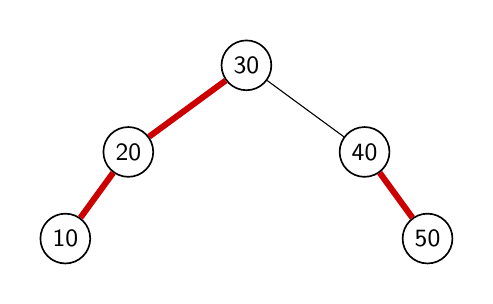
\begin{tikzpicture}[level distance=1.1cm,
    level 1/.style={sibling distance=3cm},
    level 2/.style={sibling distance=1.6cm}]
  \node [no] {30}
  child { node [no] {20}
      child { node [no] {10} edge from parent [lv] }
      child [missing]
      edge from parent [lv]
    }
  child { node [no] {40}
      child [missing]
      child { node [no] {50} edge from parent [lv] }
    };
\end{tikzpicture}


% 4. Árvore B de ordem 5: inserção do 5 em uma raiz cheia.
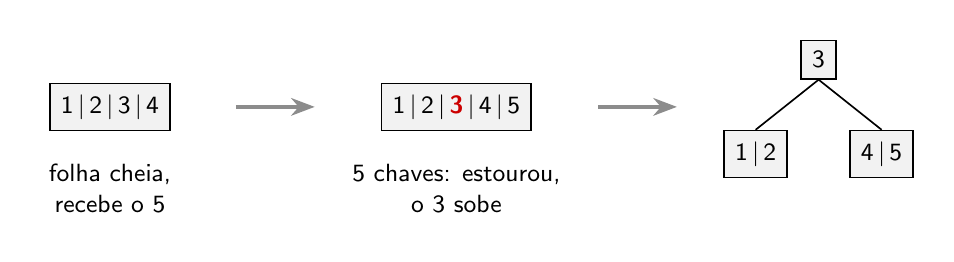
\begin{tikzpicture}
  \node [bno] (a) at (0,0) {1\sep 2\sep 3\sep 4};
  \node [rot, below=3mm of a] {folha cheia,\\recebe o 5};
  \draw [seta] (1.6,0) -- (2.6,0);
  \node [bno] (b) at (4.4,0) {1\sep 2\sep \vm{3}\sep 4\sep 5};
  \node [rot, below=3mm of b] {5 chaves: estourou,\\o 3 sobe};
  \draw [seta] (6.2,0) -- (7.2,0);
  \node [bno] (r) at (9,0.6) {3};
  \node [bno] (e) at (8.2,-0.6) {1\sep 2};
  \node [bno] (d) at (9.8,-0.6) {4\sep 5};
  \draw [lp] (r.south) -- (e.north);
  \draw [lp] (r.south) -- (d.north);
\end{tikzpicture}

% 5. Árvore B de ordem 5: inserção do 17, com a divisão propagando até a raiz.
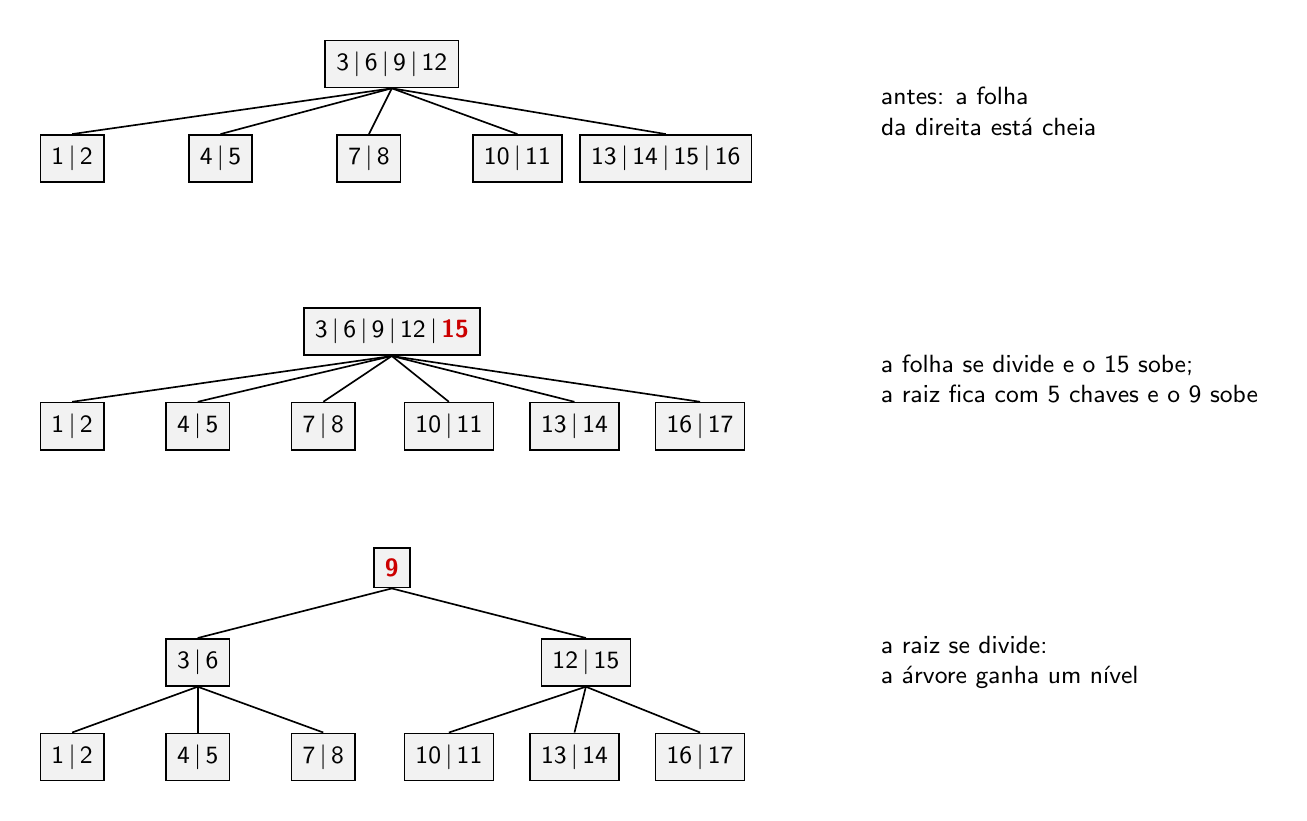
\begin{tikzpicture}[x=1.45cm]
  % antes
  \node [bno] (r) at (3,0) {3\sep 6\sep 9\sep 12};
  \foreach \t [count=\i from 0] in {1\sep 2, 4\sep 5, 7\sep 8, 10\sep 11,
      13\sep 14\sep 15\sep 16}
    \node [bno] (f\i) at (\i*1.3+0.2,-1.2) {\t};
  \foreach \i in {0,...,4} \draw [lp] (r.south) -- (f\i.north);
  \node [rot, anchor=west, align=left] at (7.2,-0.6) {antes: a folha\\da direita está cheia};

  % a folha se divide
  \begin{scope}[yshift=-3.4cm]
    \node [bno] (r) at (3,0) {3\sep 6\sep 9\sep 12\sep \vm{15}};
    \foreach \t [count=\i from 0] in {1\sep 2, 4\sep 5, 7\sep 8, 10\sep 11,
        13\sep 14, 16\sep 17}
      \node [bno] (f\i) at (\i*1.1+0.2,-1.2) {\t};
    \foreach \i in {0,...,5} \draw [lp] (r.south) -- (f\i.north);
    \node [rot, anchor=west, align=left] at (7.2,-0.6) {a folha se divide e o 15 sobe;\\a raiz fica com 5 chaves e o 9 sobe};
  \end{scope}

  % a raiz se divide
  \begin{scope}[yshift=-6.8cm]
    \node [bno] (r) at (3,0.4) {\vm{9}};
    \node [bno] (i0) at (1.3,-0.8) {3\sep 6};
    \node [bno] (i1) at (4.7,-0.8) {12\sep 15};
    \draw [lp] (r.south) -- (i0.north);
    \draw [lp] (r.south) -- (i1.north);
    \foreach \t [count=\i from 0] in {1\sep 2, 4\sep 5, 7\sep 8, 10\sep 11,
        13\sep 14, 16\sep 17}
      \node [bno] (f\i) at (\i*1.1+0.2,-2) {\t};
    \foreach \i in {0,1,2} \draw [lp] (i0.south) -- (f\i.north);
    \foreach \i in {3,4,5} \draw [lp] (i1.south) -- (f\i.north);
    \node [rot, anchor=west, align=left] at (7.2,-0.8) {a raiz se divide:\\a árvore ganha um nível};
  \end{scope}
\end{tikzpicture}

% 6. Árvore B+: separadores nos nós internos, chaves nas folhas encadeadas.
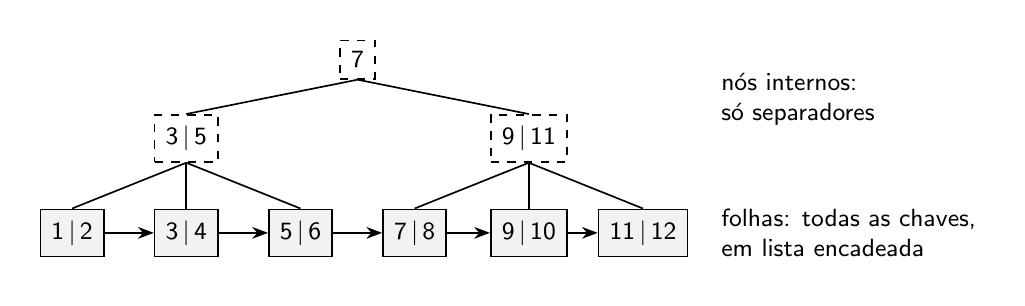
\begin{tikzpicture}[x=1.45cm]
  \node [bsep] (r) at (2.5,1.6) {7};
  \node [bsep] (i0) at (1,0.6) {3\sep 5};
  \node [bsep] (i1) at (4,0.6) {9\sep 11};
  \draw [lp] (r.south) -- (i0.north);
  \draw [lp] (r.south) -- (i1.north);
  \foreach \t [count=\i from 0] in {1\sep 2, 3\sep 4, 5\sep 6, 7\sep 8,
      9\sep 10, 11\sep 12}
    \node [bno] (f\i) at (\i,-0.6) {\t};
  \foreach \i in {0,1,2} \draw [lp] (i0.south) -- (f\i.north);
  \foreach \i in {3,4,5} \draw [lp] (i1.south) -- (f\i.north);
  \foreach \i [evaluate=\i as \j using int(\i+1)] in {0,...,4}
    \draw [prox] (f\i.east) -- (f\j.west);
  \node [rot, anchor=west, align=left] at (5.6,1.1) {nós internos:\\só separadores};
  \node [rot, anchor=west, align=left] at (5.6,-0.6) {folhas: todas as chaves,\\em lista encadeada};
\end{tikzpicture}

% 7. Trie com as 17 palavras do trie.go. Nó cinza: fim de palavra.
% O forest desenha cada nó em uma tikzpicture própria para medir, e o fundo
% branco de every picture quebra essa medição: o fundo vai só na figura final.
\begingroup
\tikzset{every picture/.style={}}
\begin{forest}
  begin draw/.code={\begin{tikzpicture}[
      background rectangle/.style={fill=white}, show background rectangle]},
  for tree={grow'=0, circle, draw, line width=0.6pt, inner sep=0pt,
    minimum size=1.5em, font=\sffamily\small, l sep=5mm, s sep=1.5mm,
    edge={line width=0.6pt}},
  fim/.style={fill=black!25},
  [raiz, rectangle, draw=none, font=\sffamily\small\itshape
    [c [a
        [r [r [o, fim]]
           [t [a, fim [z, fim]]
              [ã [o, fim]]]]
        [s [a, fim [c [o, fim]] [l, fim]]
           [o, fim]
           [s [i [n [o, fim]]]]]]]
    [d [a
        [d [o, fim [s, fim]]]
        [t [a, fim [r, fim]]]]]
    [g [r [a
        [d [e, fim]]
        [f [o, fim [s, fim]]]
        [u, fim]]]]
  ]
\end{forest}
\endgroup

% 8 a 11. Inserção em árvore 2-3 de 20, 30, ..., 80 (ver arv23.tex).
\arvDoisTresA
\arvDoisTresB
\arvDoisTresC
\arvDoisTresD

\end{document}
